\section{How to Analyze Usage Data}

When collecting usage data it is imporant to have the end in mind. How will this data be used to address the research question at hand? Not surprisingly, the nature of the collected data, especially whether it is anonymous, dramatically effects what can be learned.


\subsection{Types of Data}

\noindent
{\bf Non-anonymous data} (TODO: is there a better term for this?!), where sensitive information including source code snippets, change-sets, and even access to the source code base, provides obvious advantages. Researchers can replay developers' activity stream, affording them a deep understanding of the developer's actions~\cite{UseDisuseMisuseRefactoringsExtendedVersion}. There are few limits on how this data can be analyzed, and {\bf non-anonymous data is well-suited for exploratory studies}. Unfortunately, there are some key disadvantages. First, only developers working on open source systems are likely to participate; typical enterprise developers may face termination if they were to leak even parts of their source code base. Second, while playback is now possible, analyzing this data can be costly in terms of time and resources. 

\vspace{0.1in}

\begin{figure*}[t]
 \centering
\includegraphics[width=1\columnwidth]{Graphics/activityLogTheoretical.pdf}
%\caption{Pairwise matches across categories, including matching and mismatching pairs.}
\label{fig:theoretical}
\end{figure*}

\noindent
{\bf Anonymous data}, where only records of activities and anonymous facts about artifacts are recorded, may at first seem strictly inferior. Indeed there are some limitations around what can be inferred from anonymous activity streams. Yet the advantages make it a great complementary data source. First, developers are receptive to data collection for research purposes, and thus the ability to collect a large amount of information from many developers increases greatly. Second, because of this larger collection, while it may be more difficult to analyze anonymous data, any conclusions made on a larger data set collected from working developers are ultimately more believable, as they represent actual field usage. 

In this section we focus on analyzing anonymous data sources. We do so because analyzing anonymous activity streams is similar to analyzing non-anonymous data streams (i.e., they are both activity streams) and because the unlimited variation of analysis permitted by non-anonymous data affords few generalities. As we discuss analyzing usage data we start with straightforward magnitutde analysis, build to a categorization system for activity streams, and finally discuss dividing streams into sessions. 

%Do we need to define what kind of data can be collected?
% data = <time> <activity> <fact>*

\subsection{Magnitude Analysis}

A major advantage of anonymous usage data is its sheer size. Deriving conclusions from thousands of hours of developers' field work is naturally more convincing than from hour-long, in-lab user studies. One of the types of questions that this data is well-suited to answer is questions about magnitude. Researchers might want to know ``How often do developers invoke the pull-up refactoring'' or ``How often is the file search invoked?''. By performing a scan of the collected logs researchers can easily calculate raw counts of these actions, yet they must be wary of a few common issues with these counts. First, in any sufficiently large set of user logs there is a small set of users that will use the feature/tool under analysis orders of magnitude more often than the general population, potentially skewing the data. Secondly, any fine-grained attempt to qualify the raw counts requires making possibly incorrect assumptions about the data. For instance, there is a temptation to report searchers per hour, yet any fine-grained time calculation requires assumptions about how time was spent between activities, which experience has taught us are often wrong. Note that coarse-grained qualification, such as searches performed per day, are possible.   

\begin{figure*}[t]
 \centering
\includegraphics[width=1\columnwidth]{Graphics/activityLogActual.pdf}
%\caption{Pairwise matches across categories, including matching and mismatching pairs.}
\label{fig:actual}
\end{figure*}


\subsection{Categorization Analysis}

Magnitude analysis is well-suited for analyzing low-level behavior, yet most research questions are at a higher level. The research question ``How often are refactorings performed?'' cannot be answered via magnitude analysis alone, as refactorings can be triggered through tens of different commands. These commands first need to be categorized, after which magnitude analysis can be used. When focusing on a concrete sub-task, such as refactoring, it may be easy to categorize activities. In this case, all refactoring commands, such as pull-up or extract method, can be classified as refactorings. However, when focusing on more general behavior, such as editing, navigating, and searching, categorizations can be difficult. It is impossible to say, for instance, from a single click in the file explorer whether that click represents a search, as the developers browses a few promising files, or a navigation, as he implicitly opens a type declaration of a variable he was just browsing. Thus, categorization at the individual action level is necessarily noisey data, which effects the strength of conclusions that can be made from it.

\begin{figure*}[t]
 \centering
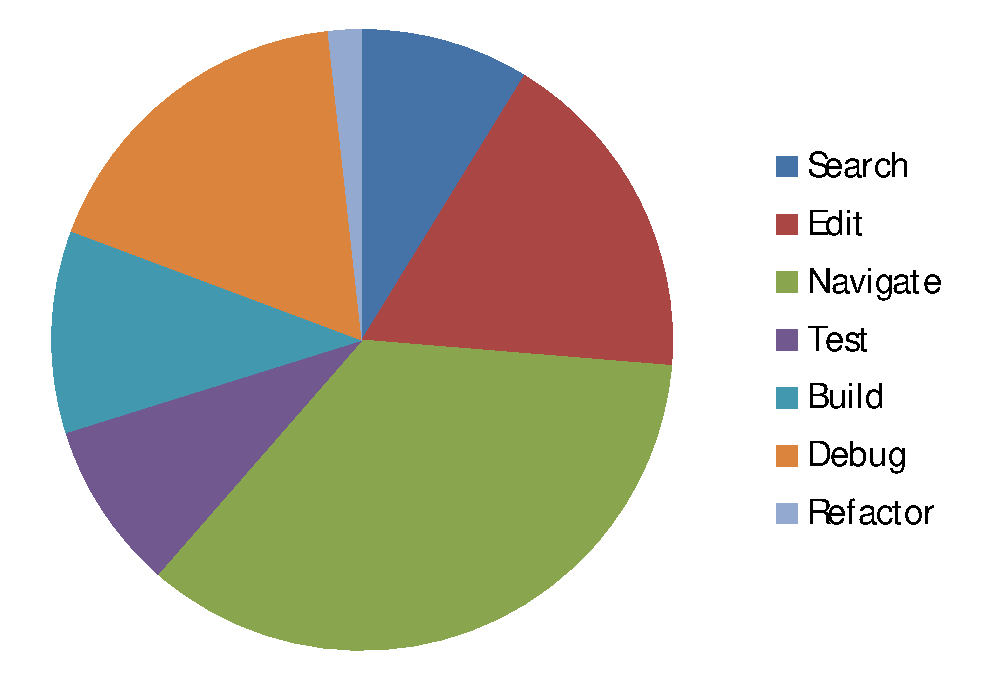
\includegraphics[width=0.5\columnwidth]{Graphics/activityCategorization.pdf}
%\caption{Pairwise matches across categories, including matching and mismatching pairs.}
\label{fig:category}
\end{figure*}


\subsection{Sequence Analysis}

Magnitude analysis and categorization both are appropriate for answering simple research questions. However, potentially the most powerful way of analyzing activity logs is through sequence analysis. 
This approach to processing logs breaks activity sequences into sessions, according to some criteria, and then reports upon characteristics of that session. Consider a researcher investigating file search. He may break activity logs into sessions, starting with a search being executed and ending on the last interaction with that result set. He could calculate additional characteristics from this raw data, such as the amount of time spent per session, the number of results reviewed, and the number of files opened.   
This type of analysis can address more complex research questions. Consider the research question ``Are users satisfied with file search results?''. This question, while impossible to answer via simple magnitude analysis can be investigated via session analysis. Using assumptions from in-lab studies that show that opening a search result followed by a long pause correlates with user satisfaction we can analyze activitiy logs to determine how often user behavior indicated satisfaction in the field. 

Sequence analysis is currently the most powerful tool we have for analyzing logs. While there has been preliminary work to complete annotate activity logs into tasks or even states (e.g., editing, searching, navigating, testing, etc.) these analyses are currently unreliable. In fact, we believe that because user behavior is often multi-purposed there will remain major obstacles to inferring higher-level user states from activity streams, ultimately limiting the usefulness of any full log analysis. 

% sequences of events
% categorization great at giving rough indication of low-level act, amoutn time
% next level is looking into characteristics of event streams
% gives better timing data and allows specific investigations
% example: refactoring, search session, test creation session, commit session
% note: similar things to non-anonymous data can be gotten from this
% identify start and end, calculate characteristics within
% example: search: time, num clicks, time spent on each click, was reformulated

% master state-machine
% tempation after considering sequences is to make a master state machine.
% note: one of the advantages of sequences is 

% Analyzing Activity Streams
%
% ex: 
%
%
  %\begin{enumerate}
  %\item Creating meaningful classification of events
	%\begin{enumerate}
	%\item
	%Activities people working on eg. testing/debugging/search/edit
	%\item
	%Establish a goal for categorization
	%\item
	%Create categories for the goal
	%\item
	%Deciding on categories when it gets hard to tell
	%\item
	%Counting time considerations, time between events, eliminating downtime/time away
	%\end{enumerate}
  %\item Defining useful and balanced sequences % (Will, Anil)
	%\begin{enumerate}
	%\item
	%Define a goal for sequencing data
	%\item
	%Sequences aligned with time or time events.  Eg. events per day or events
	%between periods of inactivity.
	%\item
	%Natural sequences such as events between builds, events between edits, events between check-ins.
	%\item
	%Creating sequences that occur along an event count boundary
	%\item 
	%Dealing with multi-event dependent sequences where the sequence may depend on detection of a cluster of events
	%\item
	%Semi-automated ways to detect tasks people working on e.g. fix bug 33 (mylin monitor) can we do it automatically?
%
  %\item  Modeling sequences with state models %(Anil)
  %Once the sequence data is collected, we have to convert the data into a meaningful representation. 
                %\begin{enumerate}
                %\item Convert sequence data to usage data : 
                %\item Calculate usage probability
                %\item Calculate transitional probability
                %\item Visualization
                %\item Data mining
                %\end{enumerate}
	%\end{enumerate}
%
  %\end{enumerate}
